\documentclass[11pt]{article}

\usepackage[margin=1.0in]{geometry}
\linespread{1.5}
\usepackage{graphicx}
\usepackage{amsmath}
\usepackage{cite}




\renewcommand{\bottomfraction}{.9}
\renewcommand{\topfraction}{.9}
\renewcommand{\textfraction}{0.1}
\renewcommand{\floatpagefraction}{.9}


\begin{document}

\section*{Introduction, Rough}

Over the years, a variety of models have been proposed to describe the effects of natural selection on protein-coding sequences, in a phylogenetic context. Traditionally, the focus has been on mechanistic codon-substitution models (see ref.~\cite{Anisimova2009} for a comprehensive review). Since their introduction in the 1990s, these models have seen great success in inferring protein evolutionary rates, or the nonsynonymous/synonymous rate ratio ($dN/dS$). This metric indicates how quickly a protein's constituent amino acids change \cite{GoldmanYang1994, MuseGaut1994, NielsenYang1998}, allowing for the identification of positively-selected regions in protein sequences \cite{ NielsenYang1998,Yangetal2000}. 

More recently, a second class of models, known as mutation-selection-balance (MutSel) models, has emerged as a popular alternative to $dN/dS$ models. Unlike mechanistic codon models, MutSel models explicitly model the dynamic balance between mutation and selection, rather than merely the final outcome (e.g. substitution) of this process \cite{HalpernBruno1998, YangNielsen2008, Rodrigueetal2010, Tamurietal2012}. Moreover, these models yield estimates of amino acid selection coefficients, which indicate the extent to which natural selection favors, or disfavors, particular amino acids at protein positions. These selection coefficients, which can in turn be scaled relative to a focal amino acid, the primary parameters of interest that MutSel models produce. Although MutSel models were first introduced over 15 years ago \cite{HalpernBruno1998}, they have seen virtually no use due to their high computational expense. However, recently, several computationally tractable model implementations have emerged \cite{RodrigueLartillot2014,Tamurietal2014}, allowing for the first time the potential for widespread use. 

Some have argued that MutSel models are more robust than $dN/dS$ and can better describe the evo process owing to their treatment of amino acid identities. More fine-grained modeling results than a $dN/dS$ analysis would yield. However, it is virtually unknown how these models really relate, so it remains unclear whether one model should be preferred over another. We don't know how parameter estimates even relate.

Although both $dN/dS$ and MutSel models describe the same fundamental process of protein evolution along a phylogeny, the relationship between these models is largely unknown. These two classes of models have largely been developed independently, and as a consequence we do not know whether parameters estimated from a $dN/dS$ model are similar, distinct, or even contradictory to those estimated from from a MutSel model of coding sequence evolution. Here, we aim to formalize the relationship between $dN/dS$ and MutSel models by examining the extent to which their focal parameters, $dN/dS$ and scaled amino acid selection coefficients, yield overlapping information about the evolutionary process. To this end, we derive a mathematical relationship between these two parameter classes, and we demonstrate that MutSel models fully embody the $dN/dS$ values. Using a simulation approach, we verify this relationship show that we can accurately estimate $dN/dS$ values using MutSel model parameter estimates, and these estimates correspond precisely to those inferred using a traditional $dN/dS$ maximum likelihood inference approach.  Importantly, we additionally show that this relationship holds only under regimes of purifying selection or neutral evolution ($dN/dS \leq 1$). Therefore, MutSel models are inherently unable to describe protein evolution under a regime of positive selection, in which $dN/dS > 1$. This result has important implications for circumstances under which MutSel model use is justified.

 


\section*{Methods}

\subsection*{Sequence simulation and omega inference}
We simulated protein-coding sequences as a continuous-time Markov
process \cite{Yang2006} according to the MutSel model proposed by \cite{HalpernBruno1998}. This model's instantaneous rate matrix $Q = q_{ij}$, which describes the probability of substitution from codon $i$ to codon $j$, is given by 

\begin{equation}
Q_{ij} = \left\{ \begin{array}{rl}
              0                                           &\mbox{multiple nucleotide changes} \\
              \mu_{ij}f_{ij}                          &\mbox{single nucleotide transversion} \\
              \kappa\mu_{ij}f_{ij}               &\mbox{single nucleotide transition} \\
         \end{array} \right.,
\end{equation} where $\mu_{ij}$ is the symmetric nucleotide mutation rate and $f_{ij}$ is the fixation probability from codon $i$ to $j$. The fixation probability is defined as \begin{equation}f_{ij} = ln\bigg{(}\frac{\pi_j\mu_{ij}}{\pi_i\mu_{ji}}\bigg{)}\bigg{/}\bigg{(}1 - \frac{\pi_i\mu_{ji}}{\pi_j\mu_{ij}}\bigg{)},\end{equation} where $\pi_i$ is the equilibrium frequency of codon $i$.

For each simulation, we simulated selection coefficients $s_a$ for each amino acid $a$ by drawing from a normal distribution $\mathcal{N} \sim (0, 1)$. Using these selection coefficients, we derived steady-state amino acid frequencies $F(a)$ according to the Boltzmann distribution, \begin{equation} F(a) = \frac{e^{s_a\beta}}{\sum_b e^{s_b\beta}} \end{equation}, whose denominator sums over all 20 amino acids \cite{SellaHirsh2005, Ramseyetal2011}. We selected the coefficient $\beta$, which imposes the level of constraint on amino acid frequencies, from $\mathcal{U} \sim (1.0, 3.0)$. Higher levels of $\beta$ indicate increased constraint; as this value approaches infinity, only a single amino acid will effectively have a non-zero frequency.

Once a set of 20 frequencies were derived, we assigned them to amino acids as follows. For each set of frequencies, we determined the number of preferred amino acids, defined as the number of frequency values greater than 0.05, or the frequency one would expect under neutral evolution.  We then selected a set of preferred amino acids such that the mean pair-wise Grantham scores among these amino acids was $\leq 100$. These amino acids were then randomly assigned to have the frequencies above 0.05, and the remaining amino acids were assigned randomly to all frequencies below 0.05. The resulting amino acid frequencies were then converted to codon frequencies such that all synonymous codons shared the same frequency (i.e., there was no codon bias).

All simulations were conducted along 2-taxon tress with branch lengths and all $\mu_{ij}$ values fixed at 0.005 and $10^{-6}$, respectively. This 2-taxon framework effectively represents a single evolutionary trajectory of protein evolution, which is the evolutionary scenario used by Sella and Hirsh \cite{SellaHirsh2005}. Unless otherwise stated, we simulated alignments of one-million positions. Moreover, a single evolutionary model was applied to all positions in the simulated sequences, meaning that we did not incorporate any site-wise variation into the evolutionary process. 

For each simulated alignment, we inferred $dN/dS$ values in two ways; first, we derived a $dN/dS$ value using the mathematical relationships described in \eqref{eq:fi}--\eqref{eq:dN}, and second, we used the standard maximum likelihood M0 model, which uses the GY94 evolutionary model \cite{GoldmanYang1994}, as implemented in HyPhy \cite{KosakovskyPondetal2005}. The GY94 model includes two primary parameters, $\omega=dN/dS$ and $\kappa$. \textbf{Not true, but still need explanation for why we aren't doing it:For each inference, we fixed $\kappa$ to the known simulated value}. Unless otherwise stated, we specified that HyPhy use equal equilibrium codon frequencies, such that each codon had a frequency of $1/61$. This frequency specification was necessary to achieve accurate $dN/dS$ maximum likelihood estimates, and is discussed more in depth in Results. 

To investigate the influence of codon frequency specifications, we specified three types of codon frequency specifications to HyPhy inferences: equal codon frequencies, F3x4 codon frequencies, and true codon frequencies.

\section*{Results}


\section*{Mathematical relationship between selection coefficients and omega}

\textbf{At this time, this section is largely copied from the NIH proposal, except with unequal mu's. We can always replace this with the mu's that cancel out again, given that that's what corresponds to the proof.}

We describe here how to calculate $dN/dS$ from the parameters of a MutSel model. We assume the following: (i) the mutational process is symmetric, such that $\mu_{xy}=\mu_{yx}$ for all nucleotide pairs $xy$; (ii) all synonymous codons for a given amino acid have the same fitness; there is no synonymous rate variation or codon bias.

In the framework of a MutSel model, we can write the steady-state frequency of codon $i$ as
\begin{equation}\label{eq:fi}
 f_i=e^{s_i}\Big/\sum_k e^{s_k}\,,
\end{equation}
where the sum in the denominator runs over all 61 sense codons \cite{SellaHirsh2005}. Here, $s_i$ is the \emph{scaled selection coefficient} for codon $i$; larger $s_i$ correspond to higher frequencies of codon $i$. The fixation probability for a mutation from $i$ to $j$ is \cite{HalpernBruno1998,SellaHirsh2005}
\begin{equation}\label{eq:pi}
  \pi_{i\rightarrow j} = \frac{1-(f_i/f_j)^{1/N_e}}{1-f_i/f_j}
  \approx \frac{1}{N_e} \frac{\ln f_j - \ln f_i}{1-f_i/f_j}\,,
\end{equation}
where $N_e$ is the effective population size. We can calculate an evolutionary rate by summing over all fixation probabilities weighted by the frequency of the originating codon. For example, we can write the synonymous rate $K_\text{S}$ as
\begin{equation}\label{eq:KS}
  K_\text{S} = N_e \sum_i \sum_{j \in {\cal S}_i} f_i  \pi_{i\rightarrow j}\mu_{ij}\,,
\end{equation}
where ${\cal S}_i$ is the set of codons that are synonymous to codon $i$ and differ from it by one nucleotide substitution. To normalize $K_\text{S}$, we divide it by the number of synonymous sites $L_\text{S}$, which we can calculate as 
\begin{equation}\label{eq:LS}
  L_\text{S} = \sum_i \sum_{j \in {\cal S}_i} f_i \,.
\end{equation}
Under the assumption that all synonymous codons have equal fitness (all synonymous mutations are neutral), we have $\pi_{i\rightarrow j}=1/N_e$ \cite{CrowKimura1970}, and thus we find for $dS$, the synonymous rate per synonymous site,
\begin{equation}\label{eq:dS}
  dS = \frac{K_\text{S}}{L_\text{S}}= \frac{\sum_i \sum_{j \in {\cal S}_i} f_i\mu_{ij}}{\sum_i \sum_{j \in {\cal S}_i} f_i}.
\end{equation}
Similarly, for $dN$, the non-synonymous rate per non-synonymous site, we find
\begin{equation}\label{eq:dN}
  dN = \frac{K_\text{N}}{L_\text{N}}=\frac{ N_e \sum_i \sum_{j \in {\cal N}_i} f_i  \pi_{i\rightarrow j}\mu_{ij}}{\sum_i \sum_{j \in {\cal N}_i} f_i}\,,
\end{equation}
where ${\cal N}_i$ is the set of codons that are not synonymous to codon $i$ and differ from it by one nucleotide substitution. The quantities $K_\text{N}$ and $L_\text{N}$ are defined as in Eqs.~\eqref{eq:KS} and \eqref{eq:LS} but summing over $j\in {\cal N}_i$ instead of $j\in {\cal S}_i$.

Equations \eqref{eq:fi}--\eqref{eq:dN} establish a connection between the scaled selection coefficients $s_i$ (i.e., the primary parameters of a MutSel model) and the evolutionary rate ratio $dN/dS$. 


\subsection*{$dN/dS$ values fully encapsulated by scaled selection coefficients}

To validate our derived relationship between $dN/dS$ values and scaled selection coefficients, we simulated protein-coding sequences along a lineage according to the Halpern-Bruno mutation-selection model \cite{HalpernBruno1998}. For each simulation set, we selected steady-state amino acid frequencies, which we then converted to codon frequencies, according to \begin{equation} F(a) = \frac{e^{s_a\beta}}{\sum_b e^{s_b\beta}} \end{equation}, where $F(a)$ corresponds to the frequency of amino acid $a$ and $s_a$ corresponds to the scaled selection coefficient for this amino acid. These $s_a$ values are analogous to the selection coefficient parameters which a MutSel model would infer from a given data set. For each simulation, we drew selection coefficients $s_a$ for each amino acid from $\mathcal{N} \sim (0, 1)$, and we selected the coefficient $\beta$ from \textbf{check this - $\mathcal{U} \sim (1.0, 3.0)$}. Note that higher values of $\beta$ indicate stronger constraint on the amino acid distributions; as $\beta$ approaches infinity, effectively only a single amino acid will be allowed. 

Following simulation, we calculated a $dN/dS$ value using both standard ML methods, according to the GY94 \cite{GoldmanYang1994} model, and our relationship. As shown in Figure~\ref{simple}, $dN/dS$ values derived using selection coefficients agree nearly perfectly with those inferred using standard maximum likelihood methods. We additionally demonstrate convergence of these values with increasing amounts of data, represented by simulated alignment length (Figure~\ref{conv}). We confirmed, using simulations, that this relationship holds under different model parameterizations, including different specifications for $\kappa$ (Figure~\ref{kappa}) and GC content (Figure~\ref{gc}). These results clearly show that MutSel model parameters fully encapsulate information regarding the evolutionary rate ratio, $dN/dS$, and that the results from MutSel and $dN/dS$ models are largely in agreement.



\subsection*{Maximum Likelihood inferences strongly biased by equilibrium frequency specifications}

In verifying the derived relationship between selection coefficients and $dN/dS$, we encountered some biases in ML inference methods. In particular, the specific codon frequency specification that the ML inference used had a substantial effect on its accuracy. Only when specifying equal codon frequencies (an equilibrium frequency of $1/61$ for each codon, regardless of that codon's actual frequency in the given data set) were we able to achieve agreement between our derived and ML $dN/dS$ estimates (Figure~\ref{freqspec_compare}) . On the other hand, when more commonly used codon frequency specifications, included the popular F3x4 estimator and simply using frequencies as measured from the data, ML yielded strongly inflated $dN/dS$ estimates. Indeed, as the model's codon frequency parameters were more and more tailored to the given data set, error between derived and ML $dN/dS$ values increased.

Importantly, however, our simulated data sets contained relatively constrained amino acid, and thus codon, frequencies, as a single MutSel  parameterization was applied to all positions in the simulated alignment. Therefore, we examined the extent to which codon constraints influenced this tendency for frequency specifications to yield spurious results. For each simulated alignment $i$, we calculated the Shannon entropy, \begin{equation} H(i) = - \sum_j P_j \ln P_j \end{equation}, where $P_j$ is the frequency of codon $j$ and the sum runs over all sense codons. Note that, for sense codons, the maximum $H(i) = 4.11$ value is reached when all codons have a frequency of $1/61$. We then examined the relationship between error in $dN/dS$ estimates caused by different codon frequency specifications and alignment codon entropy, as shown in Figure~\ref{freq_s_error}. Clearly, as entropy increases, thus approaching a flatter distribution of codon frequencies, error in ML estimates does indeed decrease. Even so, specifying a equal codon frequencies will nearly always minimize the error.

We contend that these results reflect a broad misinterpretation of codon frequency parameterization in mechanistic codon models. These frequencies must represent the codon frequencies which would exist \textit{in the absence of natural selection}. Selection, alternatively, acts to tune this frequencies to increase protein fitness. If one specifies equilibrium frequencies which exist after natural selection has acted on the protein sequence (i.e., frequencies measured directly from the data), then the influence of selection pressure is incorporated into these values. The desirable outcome, however, is that the $dN/dS$ parameter measures the selective strength. If other parameters in this model contain selection information, estimates for $dN/dS$ will not accurately capture selective effects.





\subsection*{Discussion}

Here, we have derived a formal mathematical relationship between the parameter estimates of MutSel and mechanistic codon models. Through a simulation approach, we validated this relationship and demonstrated that these models yield nearly identical results. However, we additionally found that MutSel models necessarily cannot describe scenarios in which positive or diversifying selection occurs, or when $dN/dS > 1$. Although it is generally acknowledged that MutSel models carry the assumption of purifying selection, we formalize and prove this result. These findings have important implications for how and when these models should be applied. In cases of purifying selection or neutral evolution, these two competing models are virtually no different from one another, and thus use of either model is fully justified. Alternatively, if positive selection is occurring, MutSel models cannot be used as they mathematically cannot capture the actual evolutionary process.

This study highlights the importance of examining the similarities and differences among different evolutionary model classes. While some may prefer one model over another, it is important to have a full understanding of why one model might be applied over another. Our results demonstrate that, for circumstances of purifying selection or neutral, the models are robust and in agreement. However, be careful, because sometimes they don't agree, and this is equally important.

Now, for the frequency specification: does this really matter? Typically, when one measures codon frequencies from the data set, codon frequencies are treated as global parameters rather than site-specific. This calculation will naturally lead to a flatter distribution of codon frequencies. 


Caveat about how our math relies on symmetric mutation rates and/or equal mutation rates, depending on which one ends up happening.
	

\subsection*{Mutation-selection-balance models are only valid for purifying selection}

\textbf{I really have no idea how to write up proofs, so I've virtually just latex'd the mathematica document. But at least the equations are there! ... next day: I'd better stop. This section might have to be yours, unfortunately.}

To show that mutation-selection models only corresponds to $dN/dS \leq 1$, we make use of that fact that each calculation of $dN/dS$, as described in equations \eqref{eq:fi}--\eqref{eq:dN}, entails summing the forward and backward fixation probabilities between codons, which are in turn divided by the codon frequency sums. We additionally assume that all mutation rates $\mu_{ij}$ are equal, and as all values for $N$ will ultimately cancel, we exclude them from the following proof. We will deal with the case of two nonsynonymous codons, $i$ and $j$, and we write their frequencies as $x$ and $y$, respectively.

As follows from \eqref{eq:pi}, the sum of the probabilities going from codon $i$ to codon $j$ and from codon $j$ to codon $i$ is \begin{equation} xP(x,y) + y(P(y,x) = \frac{2xy [\ln x - \ln y]}{x - y}\end{equation}, and we will demonstrate that this value is necessarily $\leq x + y$ for $x,y \geq 0$ and $x \leq y$.

To this end, we define the function \begin{equation} F(x,y) = x + y - \frac{2xy [\ln x - \ln y]}{x - y} \end{equation}. Thus, we show that $F(x,y) \geq 0$. For the condition $x=y$, this is straightforward to show, as $\lim_{x \to y}F(x,y) = 0$.
We now show that the first derivative of $F(x, y)$ is negative throughout $x \in (0,y)$, thus proving that $F(x, y)$ has to be monotonically decreasing, and hence $\geq0$, in this interval.

%dNdS limitations:
%One such limitation is that the $dN/dS$ parameter ignores the influence of site-specific amino acid propensities.  It is universally recognized that a particular position in a protein will only tolerate certain amino acids, due either to functional or structural constraints. However, $dN/dS$ ignores this key aspect of protein evolution and considers all nonsynonymous changes, regardless of which amino acid was substituted, as having equal weight on protein fitness, a biologically implausible assumption. An additional limitation is that codon-substitution models merely describe the result of the evolutionary process, rather than the explicit underlying mechanism producing those results. More precisely, substitutions in protein-coding sequences result from an ongoing mutation-selection balance. When a mutation occurs in a DNA sequence, natural selection must act on this mutation, either by disfavoring it, resulting in the mutation's removal from the population, or favoring it, ultimately yielding an amino acid replacement or substitution. By overlooking this underlying mechanism and focusing only on whether substitutions have occurred, codon substitution models are unable to capture the full extent of the evolutionary process. 


	
\newpage
\bibliographystyle{plos2009}
\bibliography{bibliography}	


\bigskip

\begin{figure*}[H]
\centerline{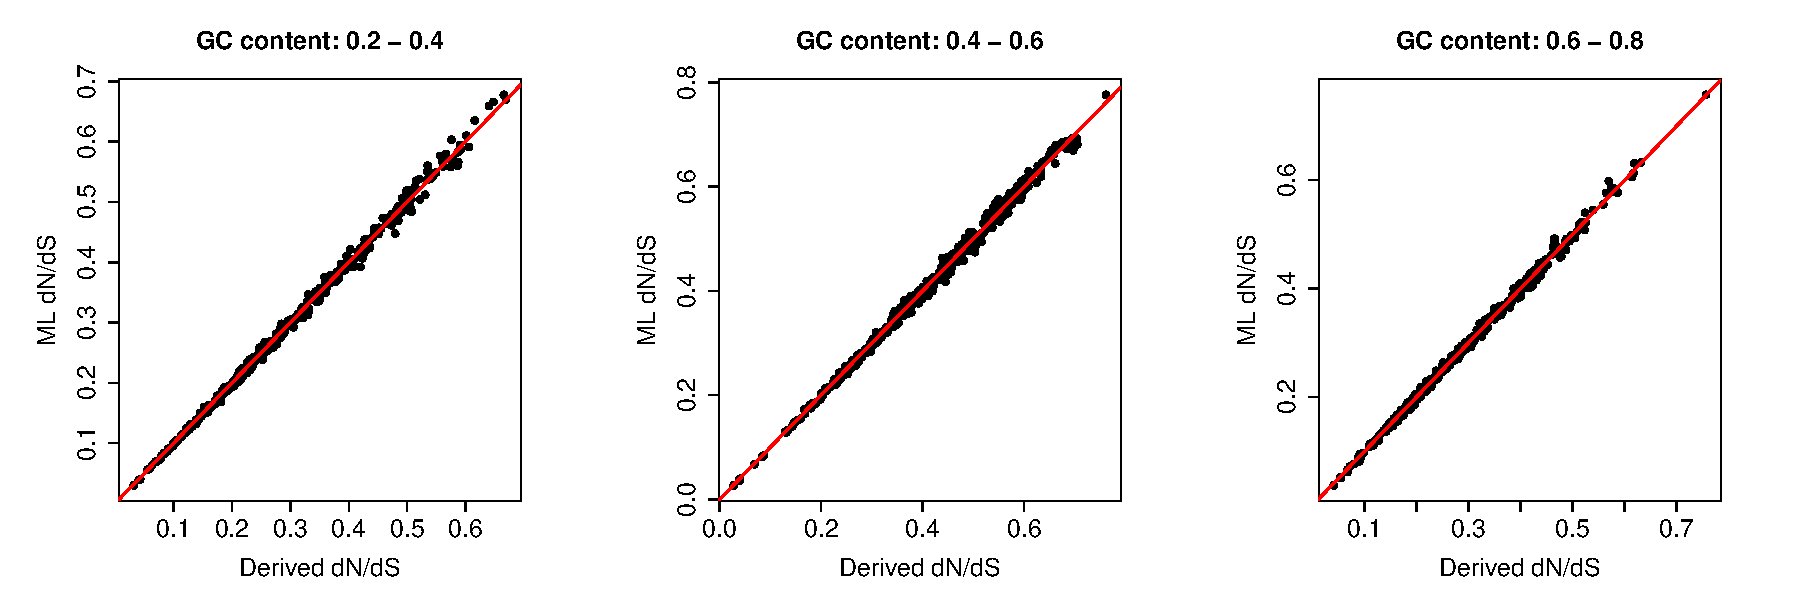
\includegraphics[width=6in]{figures/gc_2beta.pdf}}
\caption{\label{gc} GC content additionally does not influence the relationship. 400 simulations per panel.}
\end{figure*}

\begin{figure*}[H]
\centerline{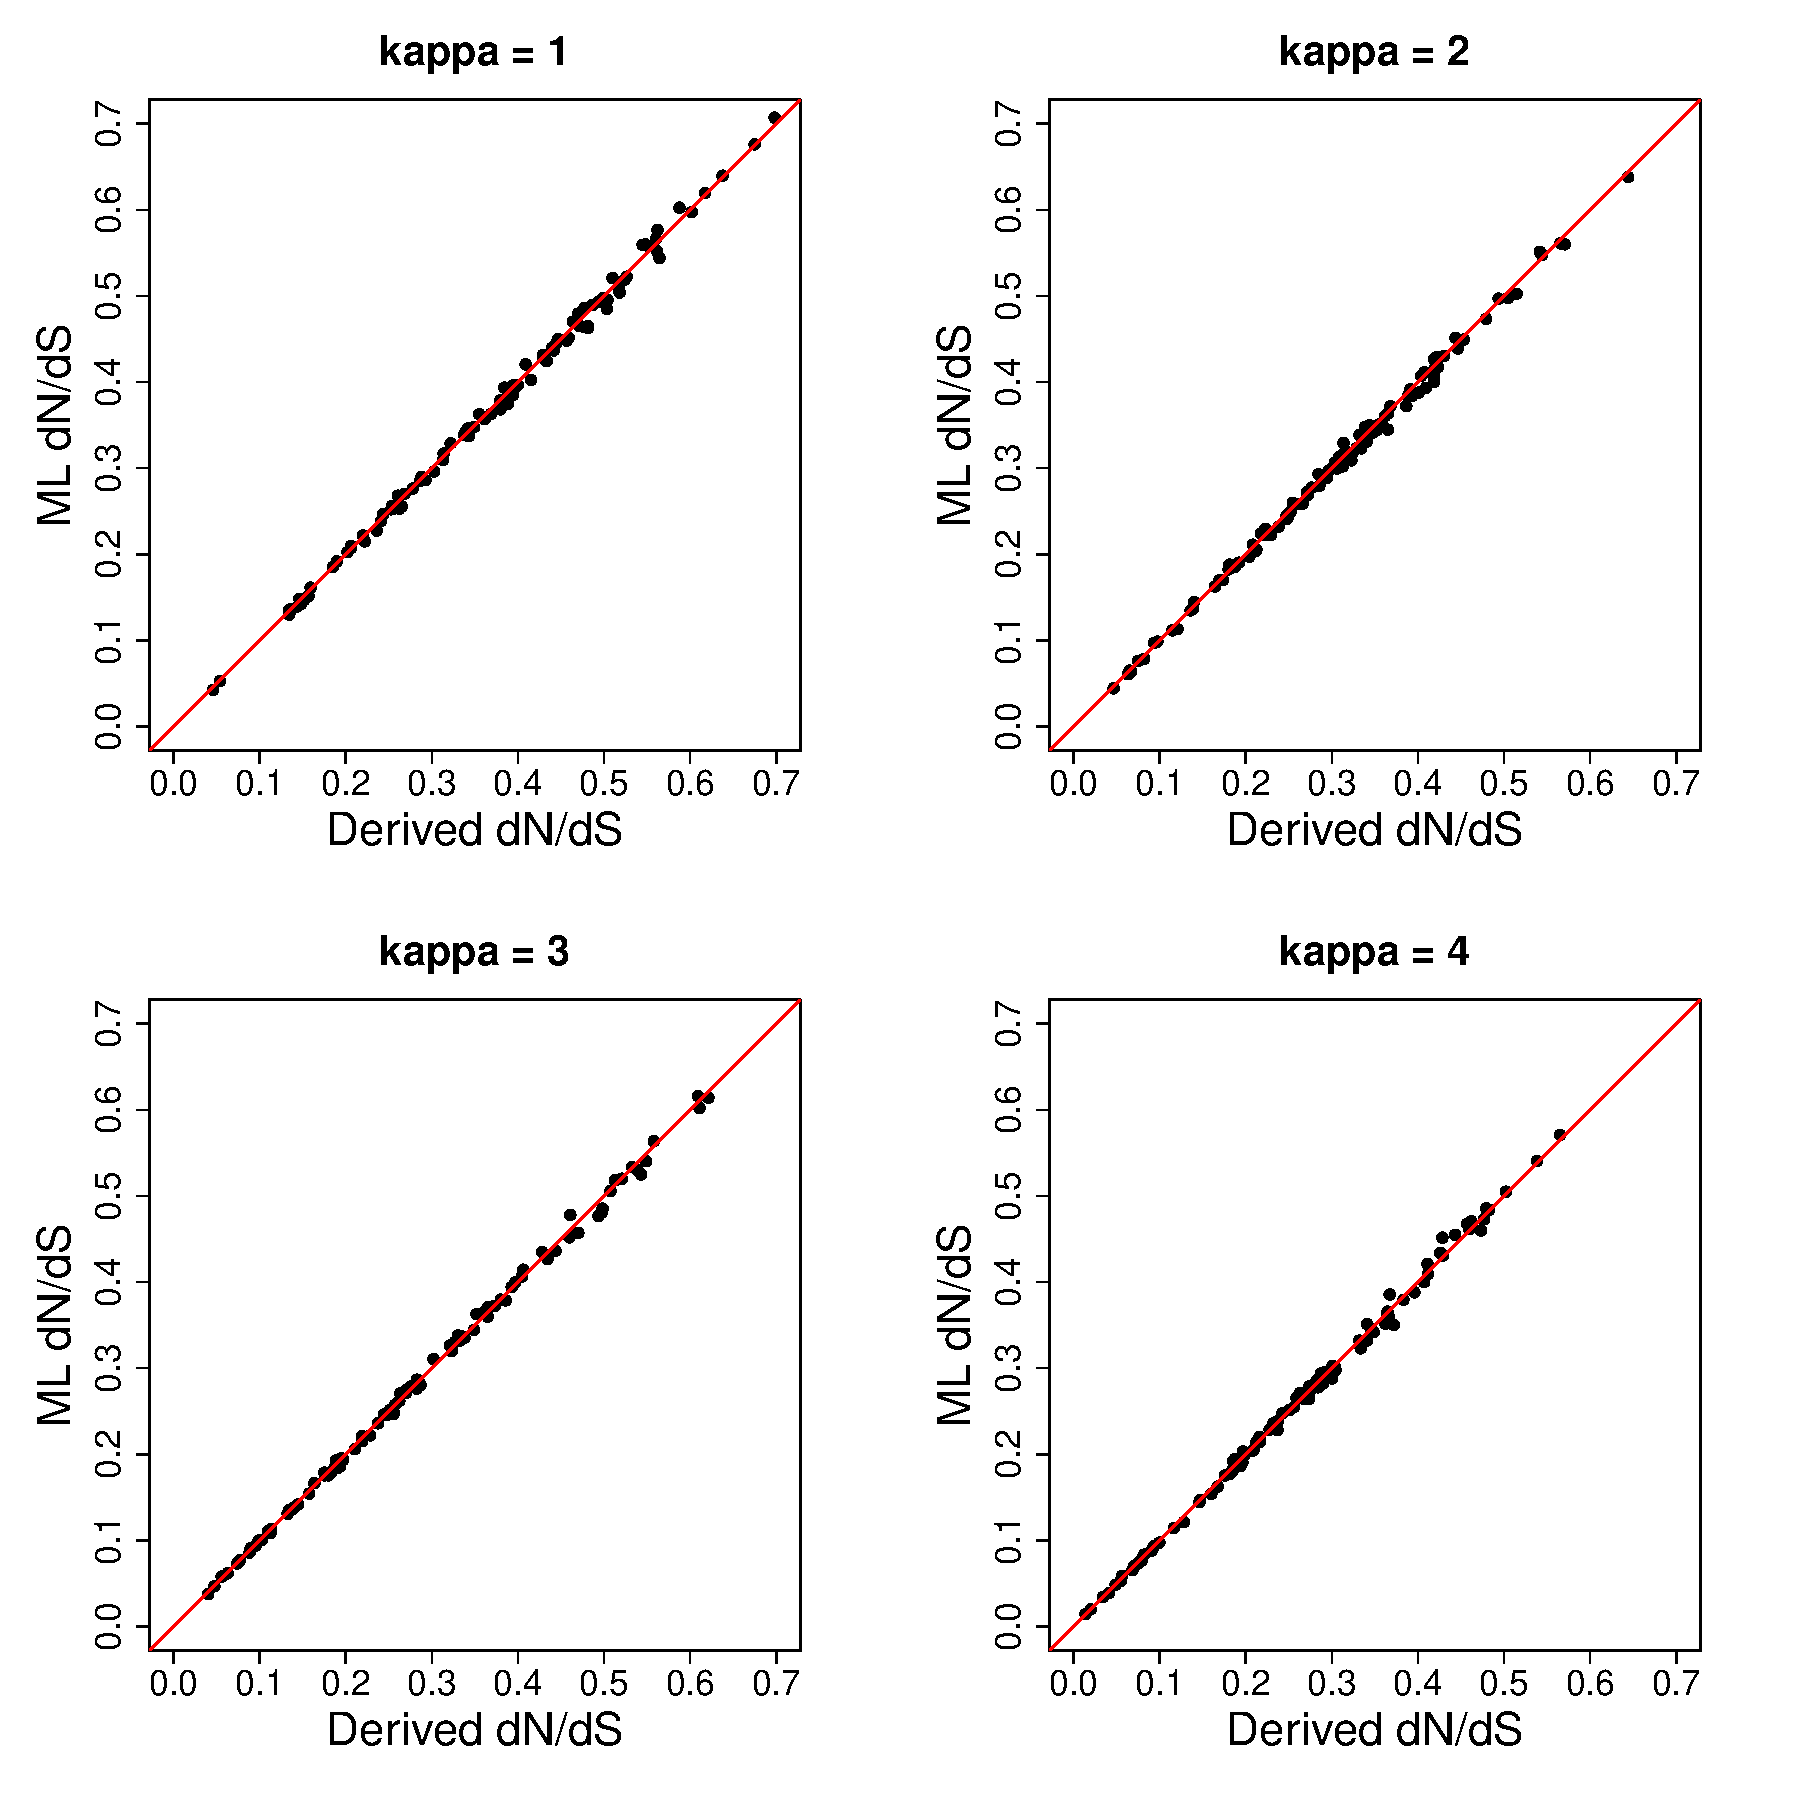
\includegraphics[width=6in]{figures/kappa_1beta.pdf}}
\caption{\label{kappa} Value of kappa does not matter for agreement with derived and ML omegas. Relationship robust to differences in (symmetric) mutational spectrum. 100 simulations per panel.}
\end{figure*}

\begin{figure*}[H]
\centerline{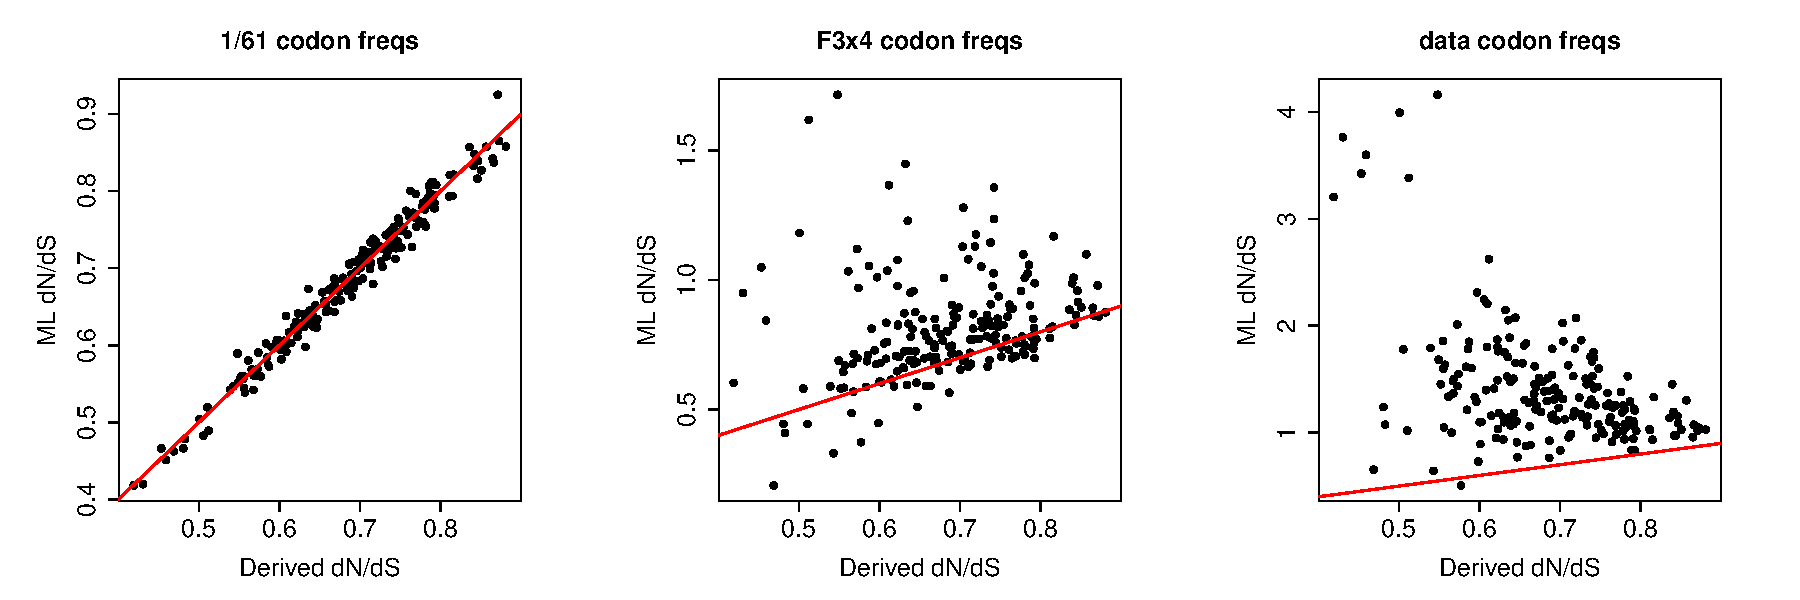
\includegraphics[width=6in]{figures/freqspec_1beta.pdf}}
\caption{\label{freqspec_compare} Equilibrium codon frequency specification to ML inference matters. Omega estimates agree when specify equal codon frequencies, and error increases as frequency specifications are more and more tailored to the data, ultimately resulting in wildly inflated values when the real frequencies are used.}
\end{figure*}

\begin{figure*}[H]
\centerline{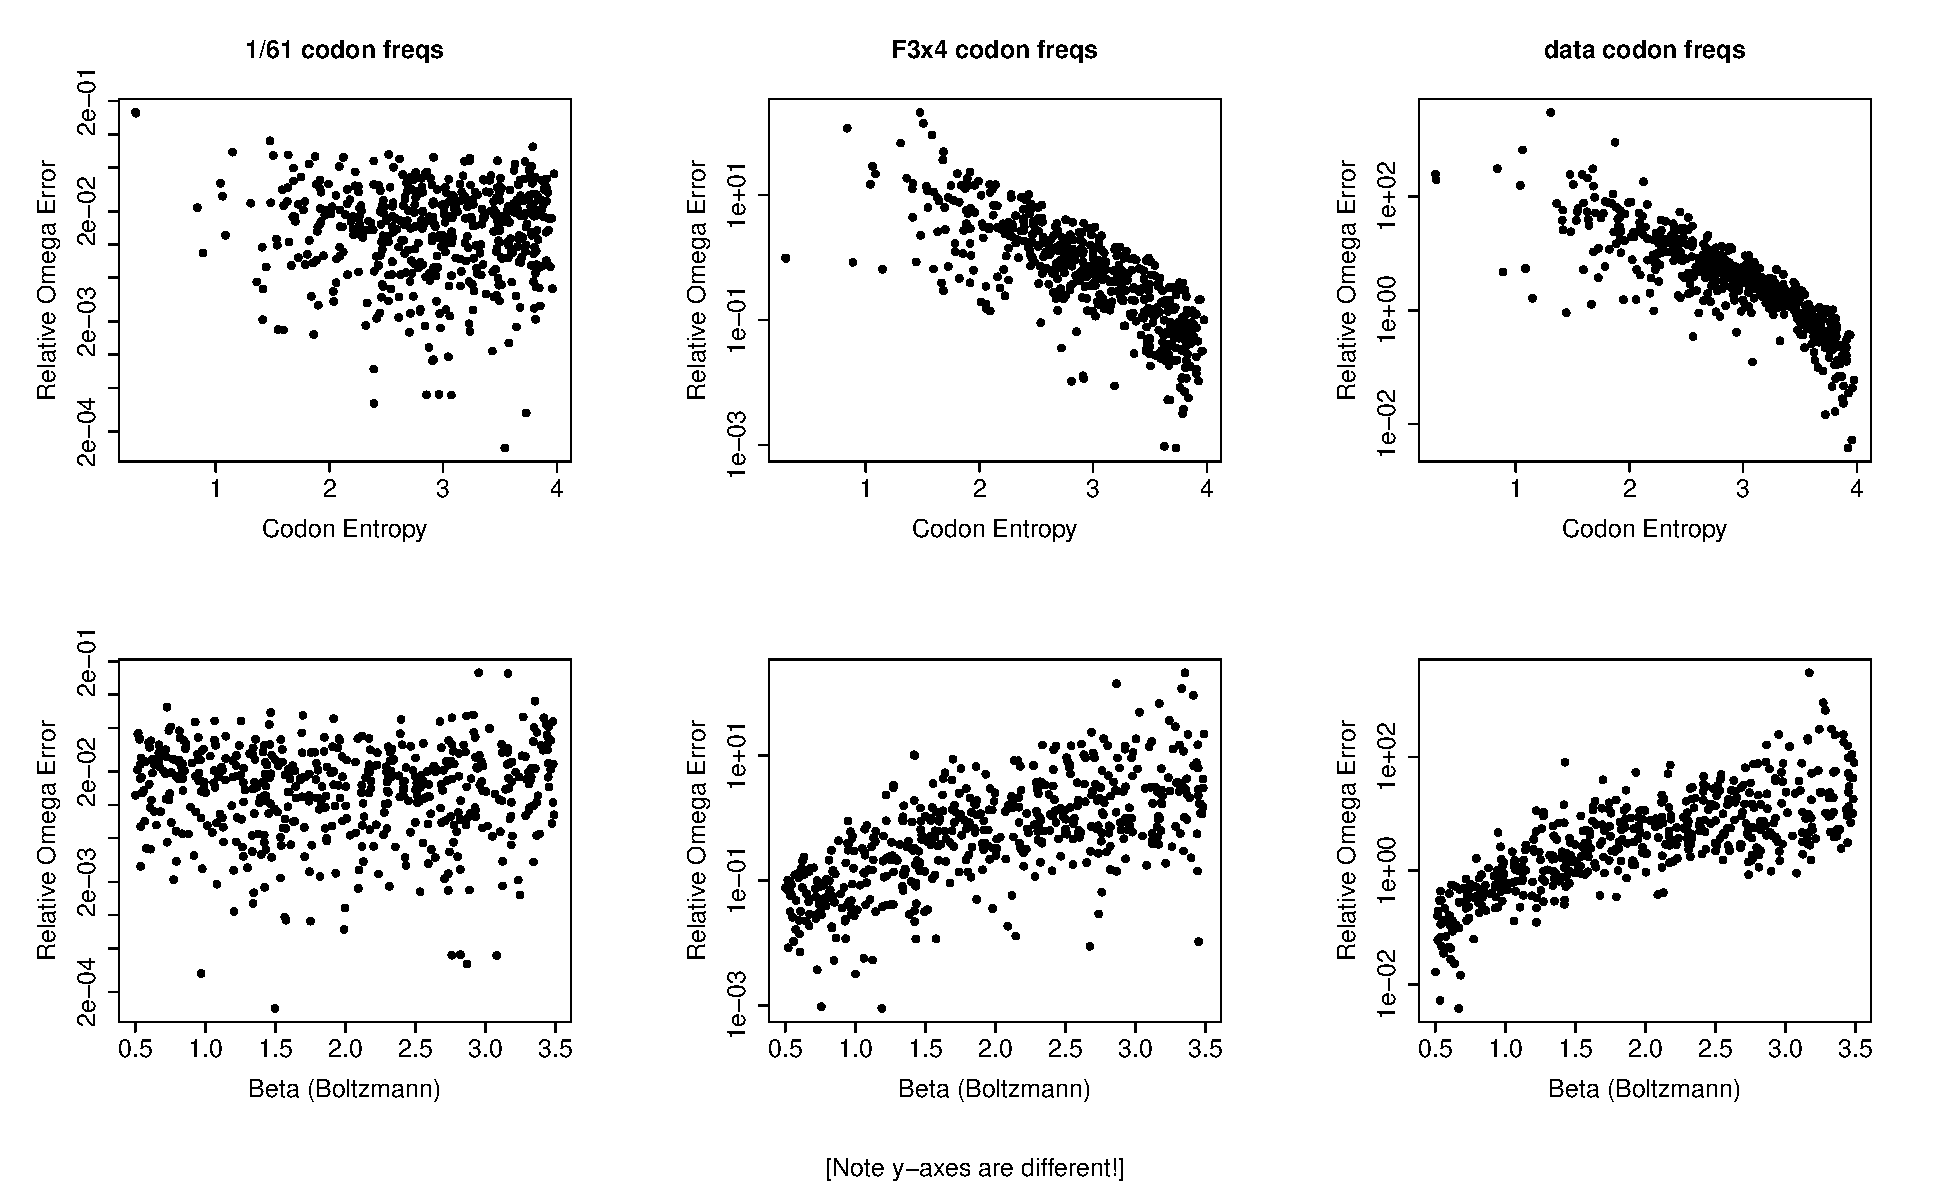
\includegraphics[width=6in]{figures/freqspec_beta_s_error.pdf}}
\caption{\label{freq_s_error} Issues with frequency specifications strongly related to the codon frequencies in the data set. Issue is more egregious when there are relatively few codons, based on entropy. As entropy increases (more permissive, and thus data set codon frequencies are flatter), the error decreases and ML more approximates the true omega value.}
\end{figure*}


\begin{figure*}[H]
\centerline{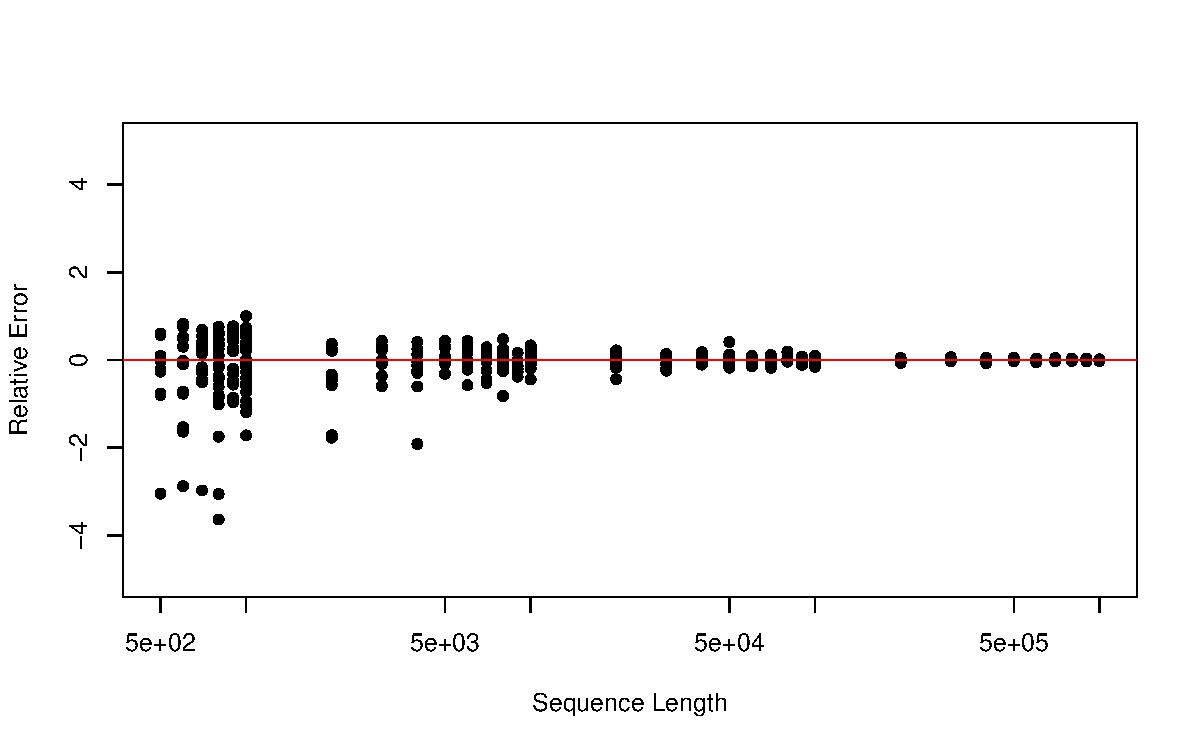
\includegraphics[width=6in]{figures/convergence.pdf}}
\caption{\label{conv} Convergence of derived $dN/dS$ and ML estimates of $dN/dS$. Each point represents results from a single simulation. The y-axis indicates relative error of the ML $dN/dS$ estimates, and the x-axis indicates sequence length on a log-scale. As the sequence length, or the data set size, increases, the two $dN/dS$ estimates converge to the same value. Note that this simulated data used a beta of 2.5.}
\end{figure*}

\begin{figure*}[H]
\centerline{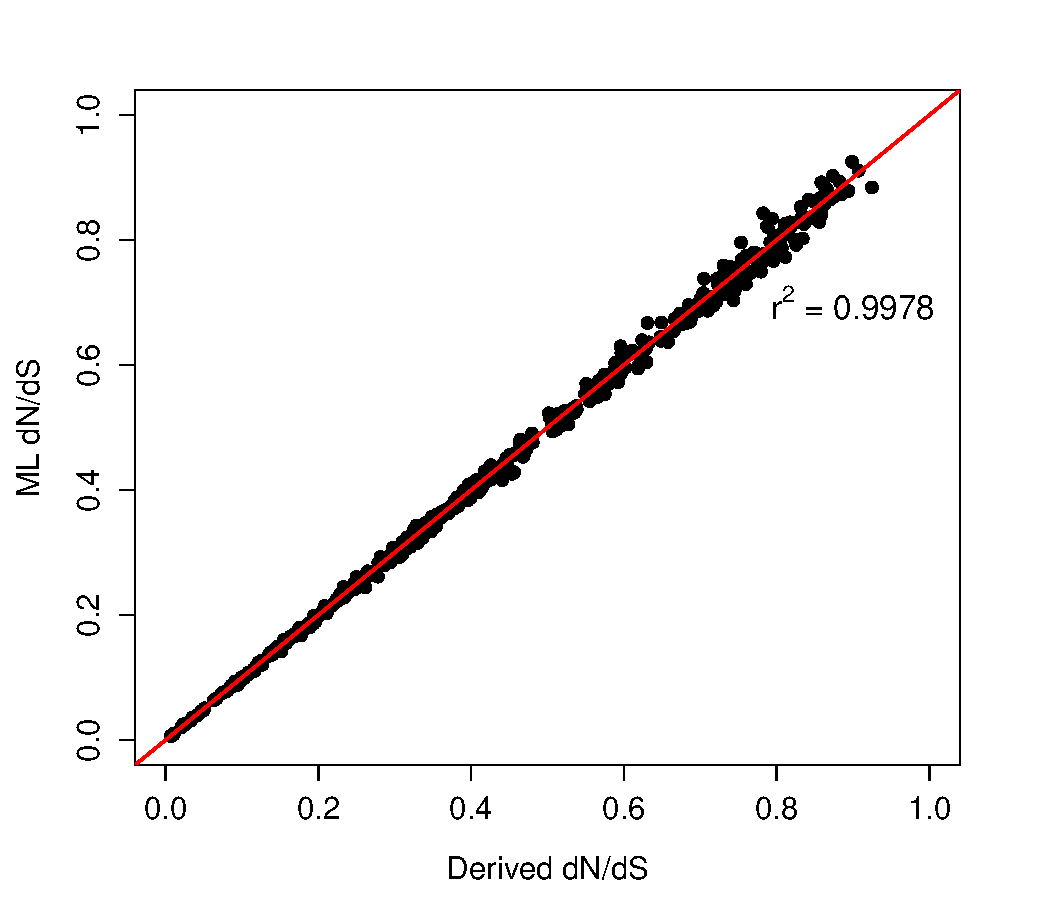
\includegraphics[width=6in]{figures/simpleregression.pdf}}
\caption{\label{simple} Relationship works exceedingly well. There are 500 points in this plot, each of which corresponds to a single simulation. Beta values for each simulation were randomly chosen between 0.5-3.5, so this plot does contain varying levels of selective constraint on amino acid distributions. Note that beta is not significant in a regression (either additive or interaction model) so the extent of constraint doesn't appear to have any influence. Moreover, kappa=1.0 here.}
\end{figure*}

	
	
	
\end{document}

